%% chapter 2

\chapter{相关工作}

\section{单细胞测序}

\subsection{什么是单细胞测序}
  人类各种组织之间细胞的类型,状态和相互作用差异巨大。而单细胞RNA测序(scRNA-seq)技术提供了在单细胞水平观测基因表达的方法,可以更好地研究这些组织及其中存在的不同类型的细胞。

  这一技术可以用于:
\begin{itemize}
    \item 研究一个组织中到底存在哪些种类的细胞
    \item 识别未知或少见的细胞类型或状态
    \item 阐明在分化过程或时间及状态变化中基因表达的改变
    \item 找出在不同条件下(如加药组和疾病组)在某一特定类型的细胞中差异表达的基因
    \item 探究一种细胞类型之间基因表达的变化,同时纳入空间,调控和蛋白质信息
\end{itemize}

  单细胞测序中解决一些较常见问题的方法\cite{liu2016single,junker2014every}包括:
\begin{itemize}
    \item 探究异质性(Studying heterogeneity)
    \item 谱系路径分析(Lineage tracing study)
    \item 随机基因表达研究(Stochastic gene expression study)
\end{itemize}

\begin{figure}[!htb]
  \centering
  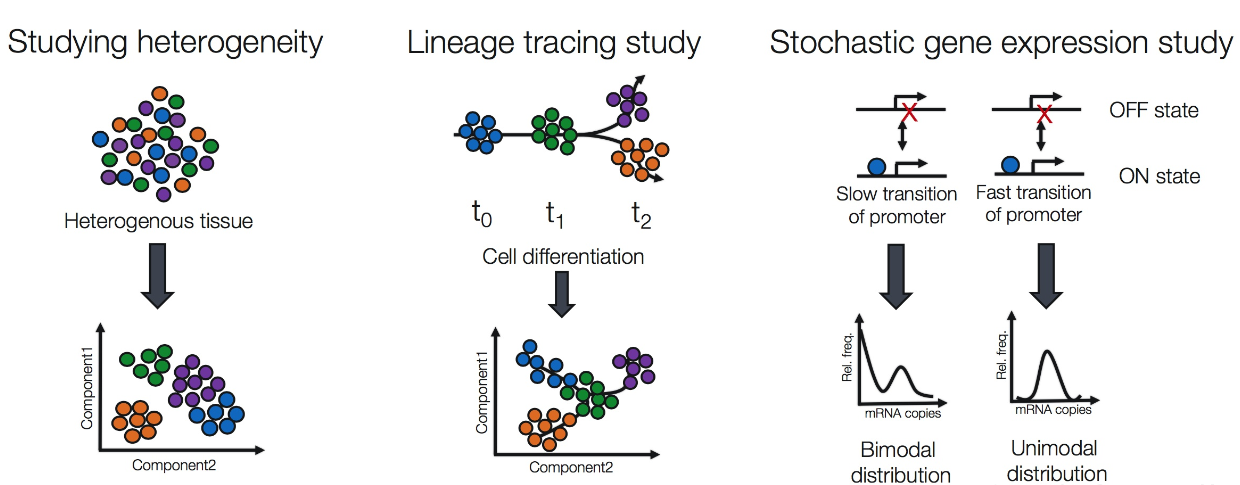
\includegraphics[width=0.8\textwidth]{figs/scseq-purpose.png}
  \caption{单细胞测序中解决一些较常见问题的方法}
  \label{fig:scseq-purpose}
\end{figure}

\subsection{单细胞测序技术的发展}
  单细胞测序技术是本课题所主要依赖的一项技术,下面将对单细胞测序技术近年来的发展进行介绍。
\begin{figure}[!htb]
  \centering
  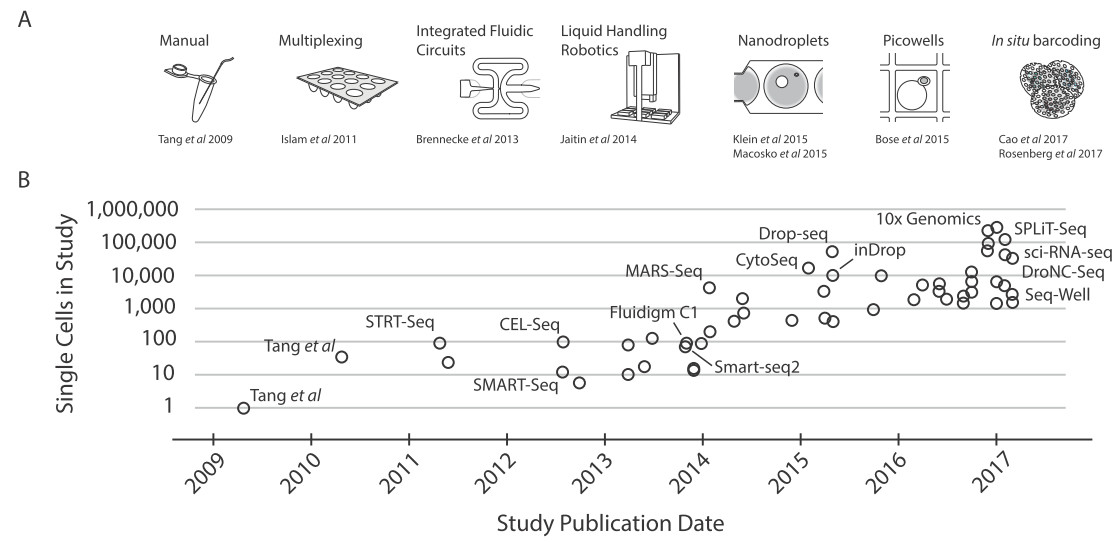
\includegraphics[width=0.8\textwidth]{figs/scseq-development.jpeg}
  \caption{单细胞测序技术近年来的发展}
  \label{fig:scseq-development}
\end{figure}

  单细胞测序技术最初起于2006年Kurimoto等人在Nucleic Acids Research上发表的一篇文章\cite{kurimoto2006improved},这篇文章对于后来单细胞转录组测序的原理发展有很大的影响。该研究主要特点在于加入了T7启动子,主要有如下两点考虑:
\begin{itemize}
    \item cDNA经历了两次扩增,分别为20个循环和9个循环,这将比直接扩增29个循环减少PCR扩增的偏差
    \item 由于试验后期并不是直接测序,而是通过T7启动子逆转录cDNA为RNA,再通过Affymetrix GeneChip Rat Genome 230 2.0 Array芯片杂交获得转录本信息。
\end{itemize}

  到2009年,汤富酬等人在Nature Methods上发表了一篇关于单细胞测序的文章\cite{tang2009mrna},正式拉开了单细胞转录组的大门。这项研究延用了Kurimoto等人在2006年工作\cite{kurimoto2006improved}在末端加A思路,但是在最后读取cDNA信息的时候,这里使用了Applied Biosystem的二代测序SOLiD system平台,也就是取代了芯片的读取方式。值得注意的是,2005年454系统问世,2007年SOLiD system问世。可以说,是二代测序成就了这篇文章。

  目前应用最广泛的是模板转换法,主要代表技术便是SMART-seq\cite{ramskold2012full,picelli2013smart},这也是我们在本课题中主要使用的测序技术。其实,在2011年的START-seq\cite{islam2011characterization},就已经用到模板转换法,同时运用Barcode标记思路来达到相对高通量的单细胞转录组测序方法。稍微改进这种方法,将Barcode加在3'端,便可以富集3'端测序,同时在一开始就将测序接头设计到引物里去,以后不用再引入,便可以做高通量。如若再不加Barcode,一个细胞的cDNA建立一个库,这样就可以获得全长的cDNA信息,也就是有了后来的SMART-seq1\&2。
\subsection{单细胞测序技术在垂体研究中的使用}
  现在,这种技术的应用范围从微生物生态系统的多样性到人类癌症的基因组学。近年来,有很多使用单细胞测序技术探究在生理、病理等状态下细胞异质性的研究\cite{hammond2019single,keren2017unique,li2019developmental,masuda2019spatial,masuda2020novel,matcovitch2016microglia}。
在关于垂体的研究中也广有使用,但以往的研究\cite{chen2020single,cheung2018single,ho2020single,fletcher2019cell}主要关注于某个发育过程中的静态分类问题,很少有研究使用单细胞转录组测序来进行动态功能研究。

  这项研究中,我们主要关注不同的垂体细胞如何响应炎症刺激。我们将基于病毒或细菌感染建立炎症小鼠模型,并主要使用单细胞转录组测序以及数据分析和数据挖掘来找出炎症、垂体和激素之间的关系,动态炎症研究将成为我们实验中最重要的部分。

  这项研究可以使我们对人体对病毒或细菌感染的免疫防御具有更清晰的认识。更重要的是,它具有非常重要的临床意义,我们希望获得用于免疫诊断的特定标记。此外,这项研究也可以为我们提供关于单细胞转录组测序技术应用的新思路。

\section{基因调控网络}

\subsection{什么是基因调控网络}
  基因调控网络(GRN)定义并维持特定于细胞类型的转录状态,这反过来又是细胞形态和功能的基础。每种细胞类型或稳定状态均由活性转录因子(TF)的特定组合定义,这些转录因子与基因组中的一组顺式调节区域相互作用(与染色质结构相互作用),以产生特定的基因表达谱\cite{fiers2018mapping,arendt2016origin}。活性TF及其靶基因的组合通常表示为GRN。

  揭露GRN是基因组研究领域的主要挑战之一。一旦确定了驱动并维持细胞状态行为的关键调节剂,它们最终就可以用来干扰这些调节程序。实例包括通过Yamanaka等人\cite{takahashi2006induction}提出的TF组合,将成纤维细胞重编程为诱导性多能干细胞(iPS),还有许多其他重编程途径,它们使用TF的特定组合将GRN从一种状态引导到另一种状态\cite{marro2011direct,ieda2010direct},以及最近在癌症治疗中的尝试,其中癌细胞被推入易受特定药物影响的状态\cite{creixell2012navigating,wouters2017decoding}。

  基于大规模转录组和表观基因组数据来计算预测GRNs是一个广泛研究的领域。相关算法包括GENIE3\cite{huynh2010inferring}、GRNBoost\cite{moerman2019grnboost2}和BEELINE\cite{pratapa2020benchmarking}等。在这项研究中我们主要使用基于GRNBoost的SCENIC\cite{aibar2017scenic,van2020scalable},进行基因调控网络推断。
\subsection{SCENIC算法原理}
  SCENIC的工作流程主要有3步:GRNBoost,基于共表达确定潜在的TF靶标;RcisTarget,进行TF基序富集分析并确定直接的靶标(调节子);AUCell,用于对单个细胞上调节子(或其他基因集)的活性进行评分。下面我们将对每一步算法原理进行介绍。
\paragraph{GRNBoost}
  GENIE3训练预测数据集中每个基因表达的随机森林模型,并将TF的表达用作输入。 然后使用不同的模型来得出TF的权重,并测量它们各自的相关性以预测每个靶基因的表达。 权重最高可以转化为TF目标监管链接。

  GRNBoost基于与GENIE3相同的概念:纯粹从基因表达矩阵中推断每个靶基因的调节子。但是,GRNBoost使用Gradient-Boosting Machines(GBM)\cite{friedman2001greedy}实现。 GBM是一种集成学习算法,它使用boosting\cite{freund1999short}作为一种策略,将浅树等多个弱学习者组合成一个强者。 这与GENIE3使用的随机森林相反,该方法使用装袋(bootstrap聚合)进行模型平均以提高回归准确性。 GRNBoost使用gradient-boosted stumps(深度为1的回归树)\cite{slawek2013ennet}作为基础学习器。

  GRNBoost的主要贡献是将这种多元回归方法转换为基于Apache Spark\cite{zaharia2012fast}的Map/Reduce\cite{dean2008mapreduce}框架。在GRNBoost中,核心数据条目是基因名称的元组和基因表达值的载体。使用Spark RDD,GRNBoost首先在计算集群中可用的节点上划分基因表达载体。随后,它构建了一个预测矩阵,其中包含所有候选调节基因的表达值。使用Spark广播变量,将预测变量矩阵广播到不同的计算分区。在框架的映射阶段,GRNBoost遍历基因元组(表达向量),并使用预测变量矩阵来训练XGBoost回归模型,并将表达向量作为各自的训练标签。从训练有素的模型中,可以得出监管者与目标之间的关系强度,并将其作为一组网络边缘发出。在缩减阶段,所有边缘集合都组合到最终的监管网络中。
\paragraph{RcisTarget}
  RcisTarget可为基因列表识别富集的TF结合基序和候选转录因子。简而言之,RcisTarget基于两个步骤。首先,它选择在基因组中的基因转录起始位点(TSS)的周围环境中显着过量表达的DNA基序。这是通过在数据库中应用基于恢复的方法来实现的,该数据库包含每个基序的全基因组跨物种排名。保留了注释为相应TF并获得归一化富集得分(NES)> 3.0的基序。接下来,对于每个基序和基因组,RcisTarget预测候选目标基因(即,基因组中排在最前沿的基因)。该方法基于Aerts等人\cite{aerts2010robust}描述的方法,该方法也可以在i-cisTarget(网络界面)\cite{herrmann2012cistarget}和iRegulon(Cytoscape插件)\cite{verfaillie2014iregulon}中实现。因此,当使用相同的参数和数据库时,RcisTarget可提供与i-cisTarget或iRegulon相同的结果,并以Janky等人\cite{verfaillie2014iregulon}中的其他TFBS富集工具为基准。
\paragraph{AUCell}
  AUCell是一种新方法,可让研究人员在单细胞RNA-seq数据中鉴定具有活跃基因调控网络的细胞。 AUCell的输入是一个基因集,输出是每个单元格中“活动”的基因集。 在SCENIC中,这些基因集是调控因子,由TF及其推定的靶标组成。

  AUCell会计算特定细胞中所有基因的排名,将其作为恢复曲线下的面积(在恢复曲线下的面积)来计算调节子的富集程度,从而根据基因的表达值对其进行排名。然后,AUCell使用AUC来计算输入基因集的关键子集是否在每个细胞的排名顶部都得到了富集。通过这种方式,AUC代表了基因签名中表达基因的比例及其与细胞内其他基因相比的相对表达值。

